\section*{Suggested Reading:}
\begin{itemize}
  %\item Bias-Variance Tradeoff: UML 5.2
  \item Bootstrap: ESL 7.11
  \item Bagging: ESL 8.7
  \item Random forests: ESL 15
  \item Boosting: UML 10
  \item Adaboost: UML 10.2, ESL 10.1

\end{itemize}

More advanced reading (beyond the material covered):
\begin{itemize}
  \item Statistical learning view of boosting: ESL 10.2, 10.4, 10.5
%  \item Optimization view of boosting - boosting as coordinate descent
  \item Gradient boosting: ESL 10.10
  \item Interpreting Boosted Trees and Random Forests: ESL 10.13

\end{itemize}

\section{Introduction}

After two lectures on theory of machine learning, we are back to new
machine learning algorithms - and specifically, 
for supervised batch learning. 
\\~\\
In the classification lecture we saw several learning algorithms for
classification. We saw that they are very different from each other - each of
them implements
a different {\bf principle} for choosing the learned rule $h_S\in\Hc$ based on the
training sample $S$, and each uses a different algorithm to implement the chosen
principle computationally - first as a formally stated algorithm, and then
actual implementation in software.
\\~\\
The classifiers we saw (eg. SVM, trees) are not ``cutting edge'' - none of them
would be considered the best choice for classification today.
%
But with the methods
of this lecture we finally get to create state-of-the-art classifiers. 
Some of the best-known
classification methods, which often that win competitions, are based on the
methods we'll see this in this lecture\footnote{For example, a list someone compiled of competitions won using
  gradient boosting: 
\url{https://github.com/Microsoft/LightGBM/blob/master/examples/README.md\#machine-learning-challenge-winning-solutions}}.
\\~\\
This lecture will be different from our classification lecture. We won't
be seeing any new learning algorithms. Instead, we will see {\bf
``meta-algorithms''}
- general methods that can be applied to any {\bf existing} learning algorithm and
improve its performance. The improvement in performance can be quite
radical. 
\\~\\
We will address classification problems for simplicity, but everything you see
here generalizes (sometimes trivially) to regression problems as well.
\\~\\  
We will learn about the three B's: {\bf Bootstrap}, {\bf Bagging} and {\bf
Boosting}. You should package these ideas together (call them $B^3$) and take
them with you wherever you go.
\begin{itemize}
  \item {\bf Bootstrap} is one of the most useful, important and influential
    ideas in statistics since computers stared being used to analyze data. It
    is  a truly magical idea that has many, many uses and applications. 
  \item One of the uses of Bootstrap is for improving prediction of a supervised
    learning algorithm. (We'll see another use in future lectures.) 
    {\bf Bagging} is a nickname for Bootstrap as it is used to improve
    prediction of a supervised
    learning algorithm.
  \item  {\bf Boosting} is another truly magical idea, which is completely
    different. And is one of the most useful,
important and influential ideas in machine learning. 
\end{itemize}
%
So, we're learning powerful
and broadly applicable ideas today.
 You'll be able to use these ideas when you
encounter difficult problems, even outside the context of the meta-algorithms we
will see today.

\subsection{Bias/Variance}

The meta-algorithms we will see in this lecture succeed because they change the
bias and the variance of the learning algorithms on top of which they are
applied. 
So, before we actually start talking about them, let us recall the {\bf bias-variance tradeoff} (also known as
the bias-complexity tradeoff). 
\\~\\
Several times in the course so far, we stated - informally - that the ``larger''
or ``more complicated'' our chosen hypothesis class, typically 
our learner will have lower
{\bf bias}
 and higher {\bf variance.}
\\~\\
 We said informally that {\bf bias} is part of the generalization error that is 
 incurred by the ``best'' hypothesis in $\Hc$. If
 we think of an unknown labeling function $f$ chosen by nature, 
 then bias measures how well the unknown labeling function $f$ can be decried by the
 ``closest'' hypothesis in $\Hc$. Obviously, the larger $\Hc$, the more
 expressive power it has to describe more complicated functions $f$ - hence a
 lower bias.
\\~\\
 We said informally that {\bf variance} is the part of the generalization error that is
 incurred by the fact that the training sample is random, hence our chosen rule
 $h_S$ is also random. The larger $\Hc$ will be, the more freedom our learning
 algorithm has to ``chase'' random fluctuations in the training sample, which do
 not represent the underlying labeling we are trying to learn. (Variance can be
   further broken down into two parts - one part comes from randomness in
   the choice of training samples, and another part comes from the measurement
 noise or noise in the labels. Let's keep in simple and not go into that now.)
\\~\\
 We mentioned the bias-variance {\bf tradeoff} - the more complicated the model,
 the smaller the bias and the larger the variance. Informally, the
 generalization error is the sum (or somehow the combination) of these two. So
 when we can tune the model complexity (another name for the size / complexity
 of our hypothesis class) we'll look for the ``sweet spot'' of a model that not
 has just the right amount of complexity, not too much and not too little.

\begin{figure}[H]
  \centering
  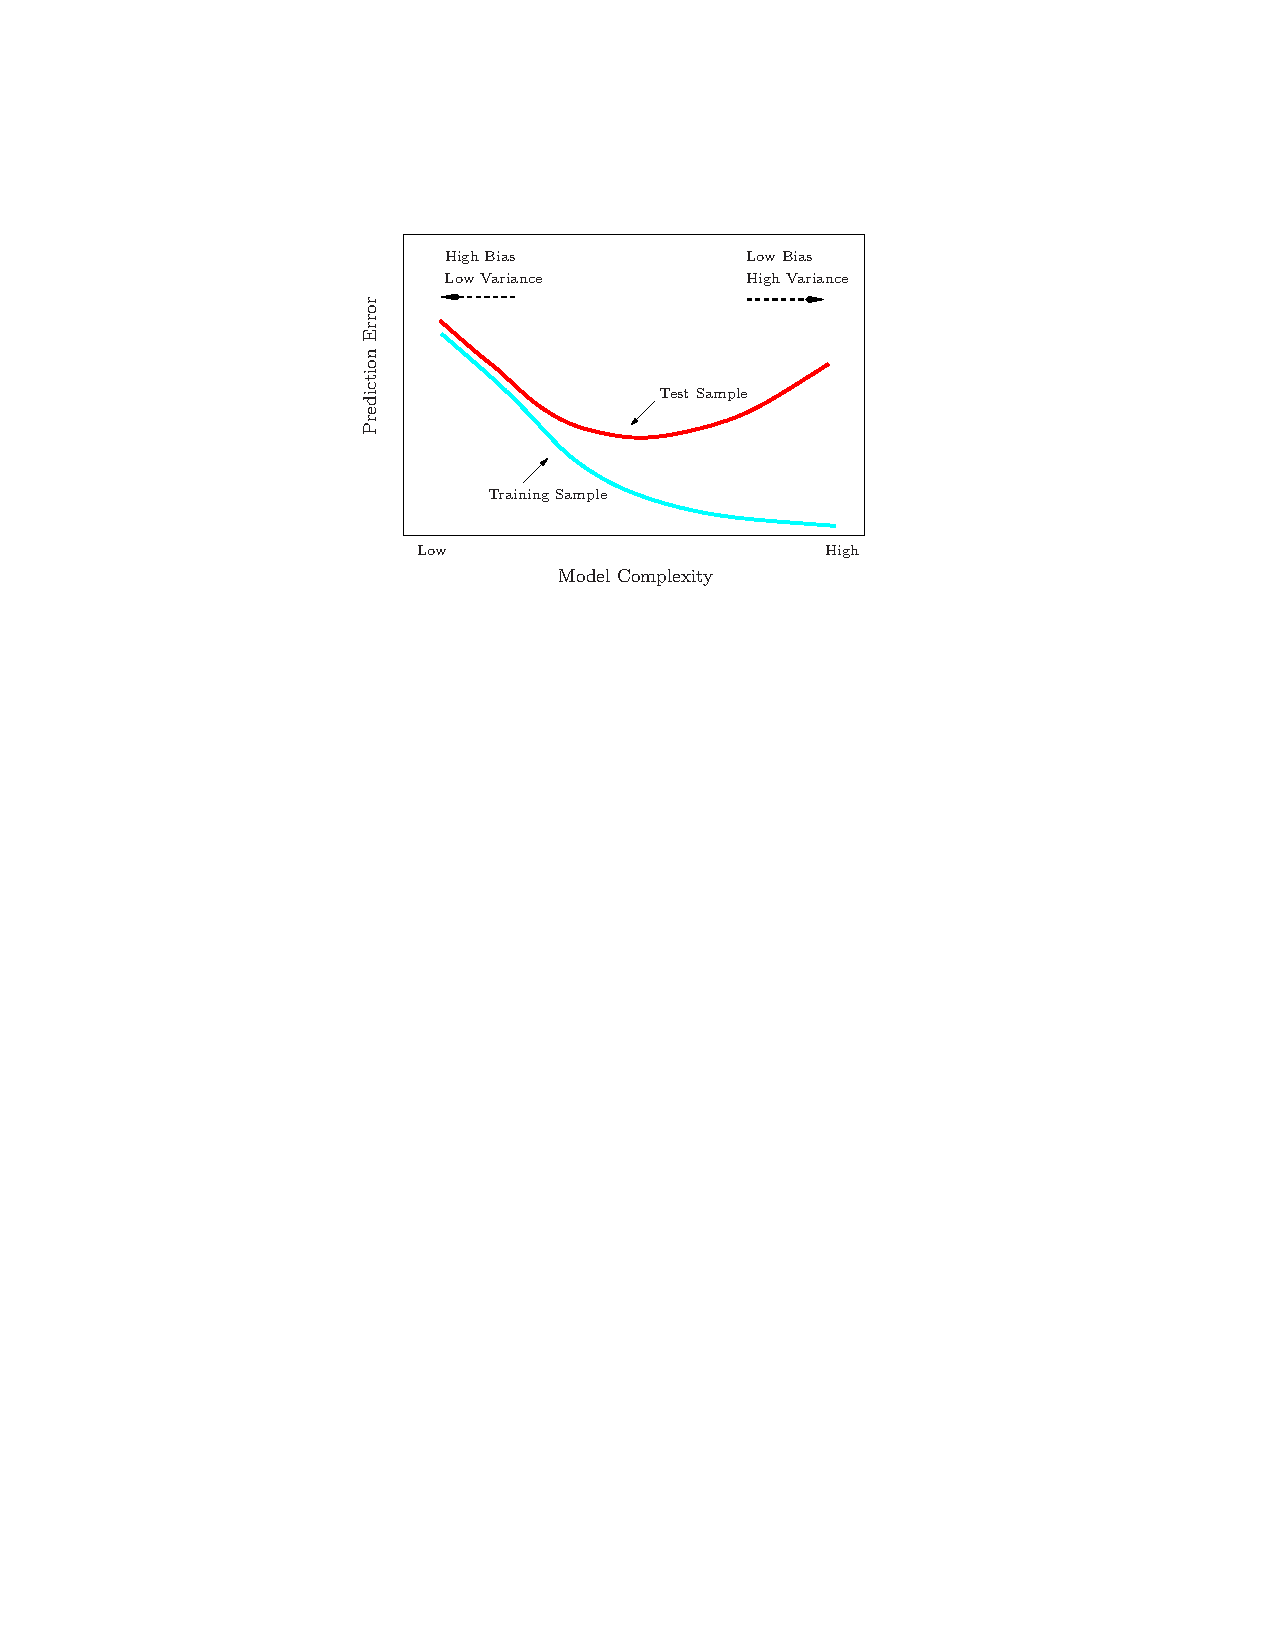
\includegraphics[width=4.5in]{ESL_bias_variance.pdf}  
  \caption{the bias-variance tradeoff}
\end{figure}

We will revisit the bias-variance more formally in one of the next lectures.
\\~\\
The magic in the methods we'll see in this lecture is that they allow us to
escape the tradeoff in a certain sense. One meta-algorithm we'll see will
reduce the bias of the learning algorithm it's applied to - without
substantially increasing its variance. The other meta-algorithm we'll see will
reduce variance without substantially increasing the bias. So, magic.

\subsection{Ensemble / Committee methods}

\begin{quote}
  ``A collective wisdom of many is likely more accurate than any one.'' —
Aristotle, in {\em Politics}, circa 300BC
\end{quote}
%
\noindent It's been known for a long time that committees typically make better decisions
than individuals. (The original Greek democracy basically comes down to this
idea.) 
\\~\\
Consider a committee of $T$ members, which has to make a yes/no decision. In
hindsight we'll know whether the decision has been right or wrong.
Each member casts her vote. Each one has probability $p$ of being correct and
probability $1-p$ of being wrong. Let's assume for simplicity that all members
are ``equally wise'', so that $p$ is the same for all members. After all members
vote, the committee's decision is simply the majority vote.
\\~\\
{\bf Exercise.} Let $X_1,\ldots, X_T$ be i.i.d Bernoulli $(p)$ random variables
taking values in $\left\{ \pm 1 \right\}$. Show that the 
above committee's random decision is given by  (when each member has equal
probability $p$ to be right) is simply 
$\overline{X}:= sign(\sum_{t=1}^T X_t)$. Conclude that the probability that the
above committee will make the right decision is $\Prob\left\{ \overline{X}>0
\right\}$.

\subsection{The uncorrelated case.}

\paragraph{Accuracy of the committee's decision.} 
It turns out that if each member is typically right ($p>0.5)$, 
then the probability that the committee is right is much higher than any
individual member, and growing with the number of committee members $T$:
%
{\bf Exercise.} Assume that all members vote {\bf independently} of each other.
What is the probability that the committee's decision is right (namely, what is
  $\Prob\left\{ \overline{X}=+1 \right\}$ as function of
$p$ and $T$? What is the limit of this probability as $T\to\infty$? Plot the
probability that the committee's decision is right over $T$, for $p=0.4,0.5,0.7,0.9$. 
(Note: A committee of fools is a terrible decision maker: Observe that if
  $p<0.5$, so that each member is usually wrong, then the majority vote
will be worse than a single vote.) 

\paragraph{Variance of the committee's decision.} 
Now we wonder if the committee makes decisions {\bf consistently}, namely, if it
votes several times - each time the entire voting process is independent of all
other times - how likely is the committee to make the same decision?
So let's consider the {\bf variability} in the committee's decision
\\~\\
{\bf Exercise.} Given i.i.d real-valued 
random variables $X_1,\ldots,X_T$, each with variance $\sigma^2$, show that the
variance of $\overline{X}:=T^{-1}\sum_{t=1}^T X_t$ is $(\sigma^2)/T$.
\\~\\
{\bf Exercise.} What is the variance of a single Bernoulli random variable
$X\sim Ber(p)$? What is the variance of the committee's vote $\overline{X}$  as
function of $T$ and $p$? plot this variance over $T$ for $p=0.4,0.5,0.7,0.9$. 



\subsection{The correlated case.}


In practice, however, committee members rarely vote independently. So let's
assume that each two members are correlated with equal correlation $0\leq  \rho
\leq 1 $. So that each member is right with (equal) probability $p$ and each pair of
members have (equal) correlation $\rho$. 

\paragraph{Accuracy of the committee's decision.} 
~\\
{\bf Exercise.} Assume every two committee members have equal correlation $\rho$
as above, and that their individual decision-making process is the same.
{\bf Use a simulation} to plot 
 the probability that the committee's decision is right (namely, what is
  $\Prob\left\{ \overline{X}=+1 \right\}$ as function of  $T$, for $p=0.7$ 
  and $\rho=0.2, 0.5, 0.9$.
  What do you think is the limit of this probability as $T\to\infty$? 

\paragraph{Variance of the committee's decision.} 
~\\
{\bf Exercise.} Given identically-distributed real-valued 
random variables $X_1,\ldots,X_T$, each with variance $\sigma^2$, and such that
$corr(X_i,X_j)=\rho$ for all $1\leq i\neq j\leq T$, show that the
variance of $\overline{X}:=T^{-1}\sum_{t=1}^T X_t$ is 
\[\rho\cdot(\sigma^2) + (1-\rho)\cdot \frac{\sigma^2}{T}
\]
\\~\\
  {\bf Exercise.} 
  {\bf Use a simulation} to plot the variance of the committee's vote $\overline{X}$ 
over $T$ 
 $T$, for $p=0.7$ 
  and $\rho=0.2, 0.5, 0.9$. What do you think is the limit of this variance as $T\to\infty$? 




  \begin{figure}[H]
  \centering
  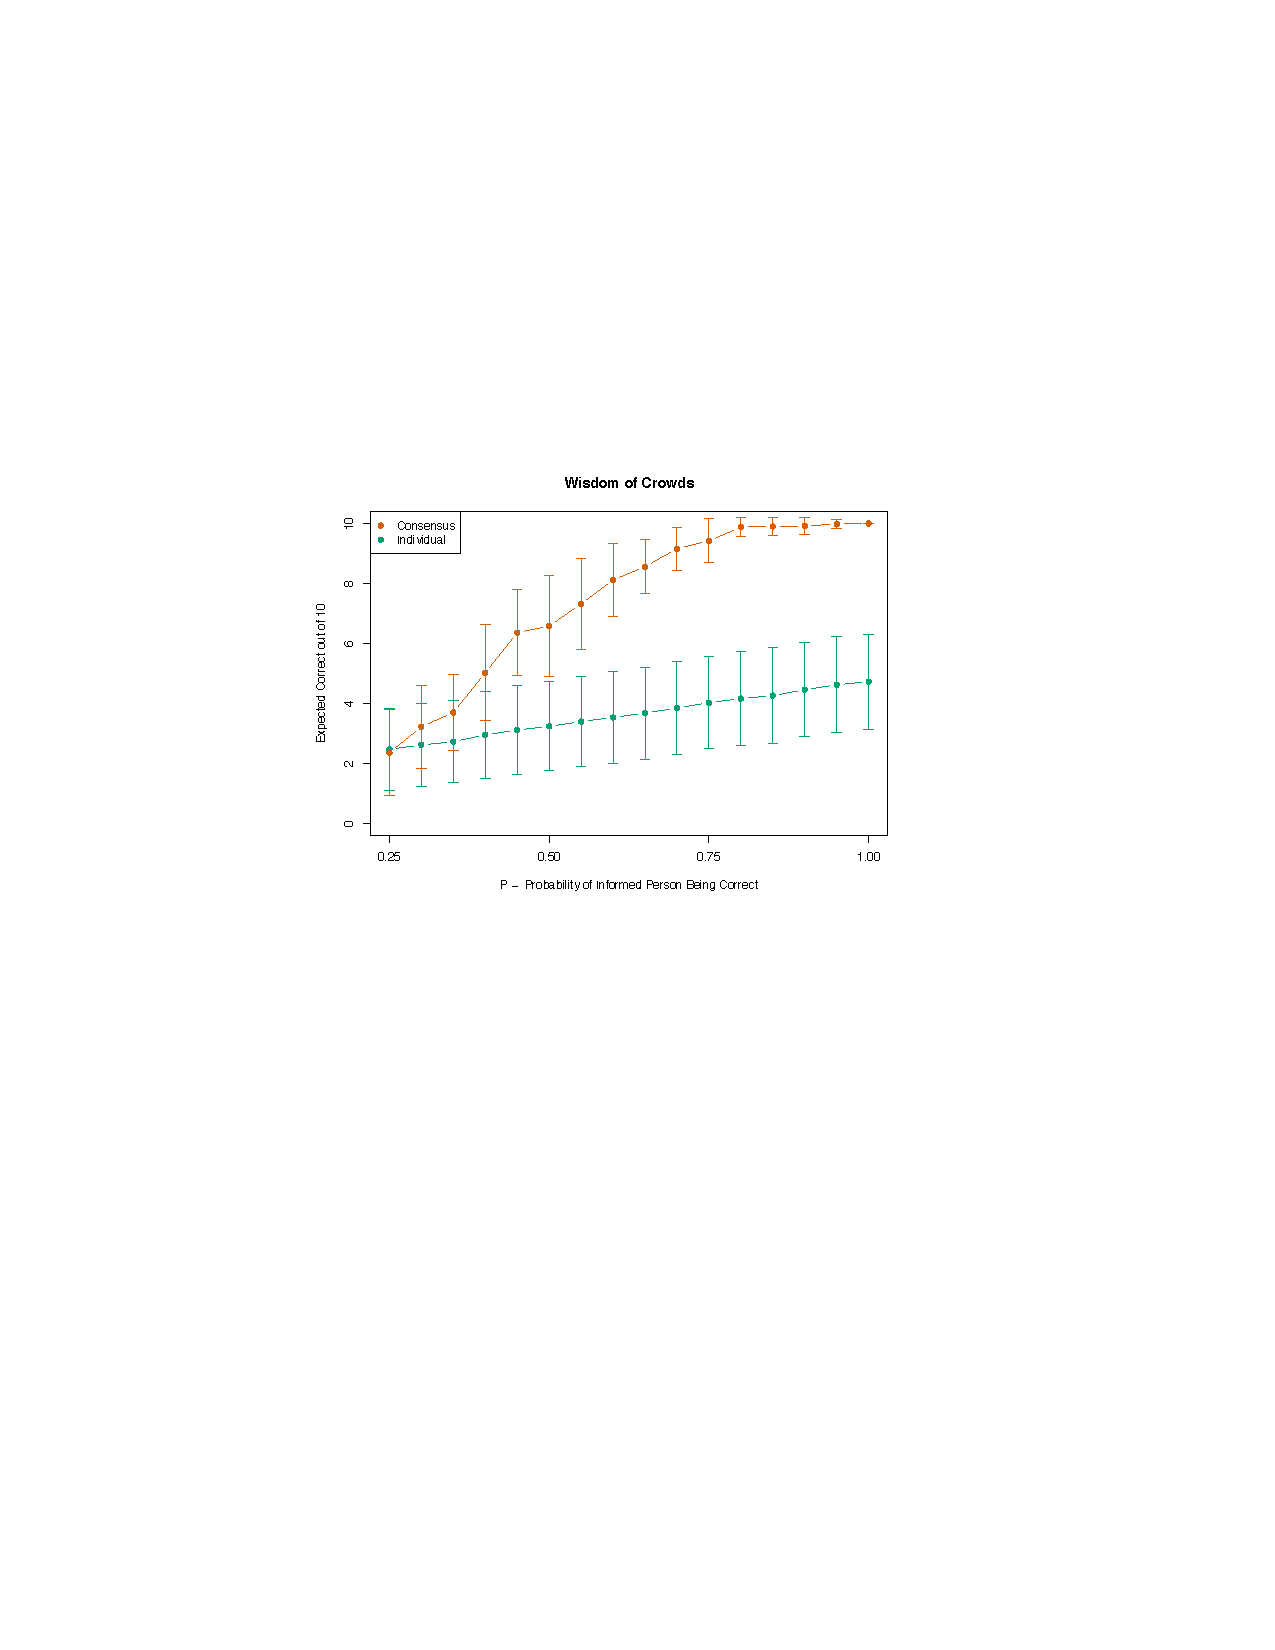
\includegraphics[width=4.5in]{crowds.pdf}  \\
  \caption{Simulation: wisdom of the crowd. The probability of the committee
    being right (and its standard deviation in errorbars) 
    overlay with the probability (and standard deviation) of each member individually being
right (ESL figure 8.11)}
\label{fig:crowds}
\end{figure}


  \subsection{Summary}

We have seen quantitatively the following general statement:
A committee of members decide by majority vote. Decisions are correlated with
correlation $\rho$ and each member is right with probability $p$. If $p>0.5$,
the committee's decision will improve with the number of members $T$ in two
ways: it has been probability of being right, and will be more consistent (less
variable). If $\rho>0$, increasing $T$ will only help up to a certain point, so
$\rho$ gives a bound on the improvement possible by moving from a single member
to a whole committee.
  



  \section{Committee methods in machine learning}

  Back to machine learning. Suppose we had $T$ training samples of size $m$ chosen
independently from $\X$ according to some distribution $\D$. Denote them by 
$S_1,\ldots,S_T$.
Suppose have a learning algorithm $\Ac$ and train it on each of the training
samples, to obtain $h_{S_1},\ldots, h_{S_T}$. The prediction $h_{S_t}(x)$ on
some sample $x\in\X$ is independent of all other predictions of the other
trained rules, and has the same distribution. So if we used  $h_{S_1},\ldots,
h_{S_T}$ in a committee - using majority vote - we have the situation from above.
The generalization loss will improve with $T$, tending to $0$ as $T\to\infty$
(if any rule $h_{S_t}$ separately has generalization loss $<0.5$).
As we saw above, the variance of the prediction will decrease as $1/T$. 
\\~\\
However, in batch learning, we don't have $T$ training samples. We just have
one. So why not train the same algorithm $\Ac$ again and again on the same
training sample $S$? well, that won't do much good - the predictions will be
identical - perfectly
correlated. 
\\~\\
So the first magic we would like to do is how to create $T$ training samples from
the one training sample $S$ we have, in a way that will mimic fresh independent
draws of new training samples of size $m$ according to $\D$. 


\paragraph{Committee methods - Definition.} 
Committee methods are {\bf ``meta-algorithms''}. 
In a committee method, we take an existing learner $\Ac$ (which we call the
  ``base'' learner, or sometimes the ``weak'' learner, for reasons we will see
below) and apply it to a
sequence of $T$ ``artificial'' training samples.
\\~\\
In this lecture we work with classification. The label set is
$\Yc={\pm 1}$ and the committee
decides by $h(x) = \text{sign} \left( \sum_{t=1}^T h_t(x) \right)$. 
Everything here applies to regression as well: in a regression problem, the
committee decides by $h(x) = T^{-1}\left( \sum_{t=1}^T h_t(x) \right)$.
\\~\\
We are going to see two very different ideas for building the committee member
rules. 
%
But After the committee is built, it is averaged the same way in all cases.
Sometimes the committee's decision will be a weighted average, to allow some
members tohave more weight than others:
$h(x) = \text{sign} \left( \sum_{t=1}^T w_t h_t(x) \right)$, 
for some  $w_t\geq 0$, $\sum w_t=1$.




\section{The Bootstrap}

Here comes the first magic. Creating new ``artificial'' training samples from
the one training sample $S$ we have seems impossible.
 But yet it actually is, and the fact that it is is one of
the most groundbreaking ideas of statistics in the 20th century. 

Given a training sample $S=\{(x_i,y_i)\}_{i=1}^m$ we are going to construct a
new training sample $S^{*1}$ as follows. We are going to sample $m$ times {\bf
with replacements} from the set $S$. The first sample we draw from $S$ will be denoted $(x^{*1}_1,y^{*1}_1)$. The second sample we draw will be denoted 
$(x^{*1}_2,y^{*1}_2)$, and so on. So we now have a sample
\[
  S^{*1}=\{(x^{*1}_i,y^{*1}_i)\}_{i=1}^m
\]
Of course, since we sampled from $S$ with replacements, there might be repeated
samples in $S^{*1}$, even if $S$ itself had no repeated samples. 
Now we can repeat this process $B$ times, obtaining $B$ training samples, each
of length $m$: $S^{*1},\ldots, S^{*B}$. The samples in the $b$-th training
sample will be denoted 
\[
  S^{*b}=\{(x^{*b}_i,y^{*b}_i)\}_{i=1}^m \,.
\]
%
\noindent This method of new training samples is called The Bootstrap, and the sample
$S^{*b}$ is called a bootstrap sample created from $S$. 

\subsection{Why does the Bootstrap work?}

Assume for a moment that samples in our learning problem are i.i.d samples from an unknown
distribution $\D$ over $\X\times \Y$. We are hoping that each Bootstrap from $S$
somehow
behaves like a fresh i.i.d sample from $\D$ itself.
\\~\\
It may seem at a first glance crazy that bootstrap samples can serve us instead
of fresh, i.i.d samples from $\D$. But in fact it is often the case. Why?
\\~\\
Given a training sample $S$ (assume for simplicity that all the points of $S$
are distinct) let's define the {\bf empirical distribution}
$\widehat{\D}_S$ induced by $S$ on $\X\times \Y$ as the following probability distribution
on $\X\times \Y$: for a subset $C\subset \X\times \Y$, define
\[
  \widehat{\D}_S( (X,Y)=(x,y) ) = 
  \begin{cases}
    \frac{1}{m} & (x,y)\in S\\ 
    0 & (x,y) \notin S
  \end{cases}
\]
or equivalently, for any $C\subset \X\times \Y$,
\[
  \widehat{\D}_S(C):= \frac{| C \cap S |}{m}\,.
\]
Observe that this is equivalent to putting a probability mass of $1/m$ on each
of the points of $S$, and zero mass on all other points in $\X\times \Y$. 
\\~\\
{\bf Now observe that a bootstrap sample $S^{*b}$ is just an i.i.d draw of $m$
points}
from the empirical distribution $\widehat{\D}_S$ induced by the one training sample we
have, $S$.
\\~\\
As $m$ grows, namely as $S$ becomes larger, the empirical distribution $\widehat{\D}_S$
converges in distribution to $\D$. The idea behind the bootstrap is that, if
$\widehat{\D}_S$ is not so different from $\D$, then $m$ i.i.d draws from
$\widehat{\D}_S$ is a good
approximation to $m$ i.i.d draws from $\D$. 
\\~\\
One way to see the convergence of the empirical distribution to the underlying
distribution is on the real line:
\\~\\
{\bf Exercise.} Let $X_1,\ldots,X_m$ be i.i.d random variables with some
distribution $F$ on the real line $\mathbf{R}$. Let $x_i\in\mathbb{R}$ be a sampled value of
$X_i$. Show that the CDF (cumulative distribution function) of this sample is a
step function, increasing from $0$ to $1$ (as all CDFs should), with jump of
size $1/m$ at each value $x_i$ (see Figure \ref{ecdf}). 
In simulation, take $F$ to be, say,
$\mathcal{N}(0,1)$. For each value $m=10,100,1000$, draw a sample and plot its
empirical CDF - and overlay the CDF of $\mathcal{N}(0,1)$. Recall that on the
real line, convergence in distribution is equivalent to convergence of the CDFs
to a limiting CDF at the continuity points of the limiting CDF.


\begin{figure}[H]
  \centering
  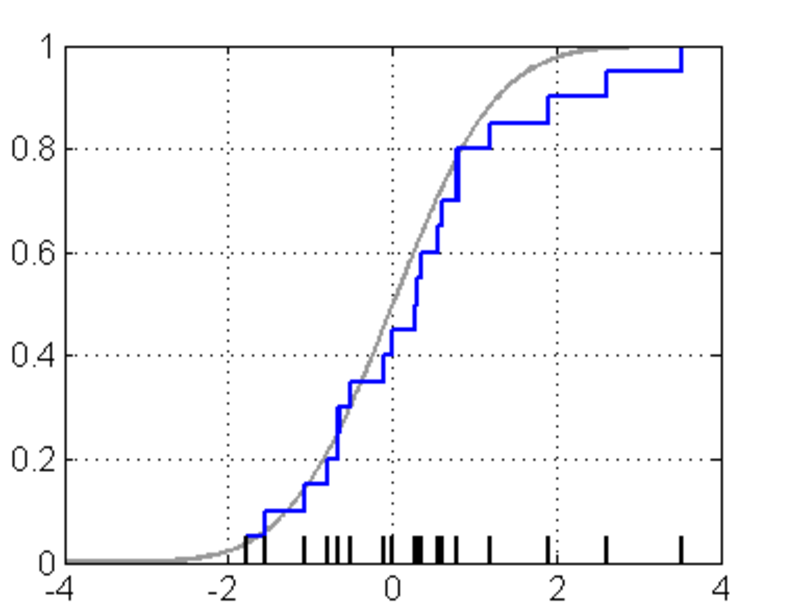
\includegraphics[width=3.5in]{ecdf.pdf}  
  \caption{CDF of a probability distribution on the real line, and empirical CDF
  of an i.i.d sample from that distribution. Black lines on the horizontal axis
show the random sample. }
\label{ecdf}
\end{figure}


%\begin{figure}[<+htpb+>]
%  \centering
%  \includof $S$ egraphics{steps}
%  \caption{<+caption text+>}
%  \label{fig:<+label+>}
%\end{figure}<++>





\noindent Why the name ``The Bootstrap''? We're seemingly creating new datasets out of nothing, as if we
were pulling ourselves up by the straps of our own boots. As you may know, there was only one man
strong enough to do that - the Baron Munchausen.

\begin{figure}[h!]
  \centering
  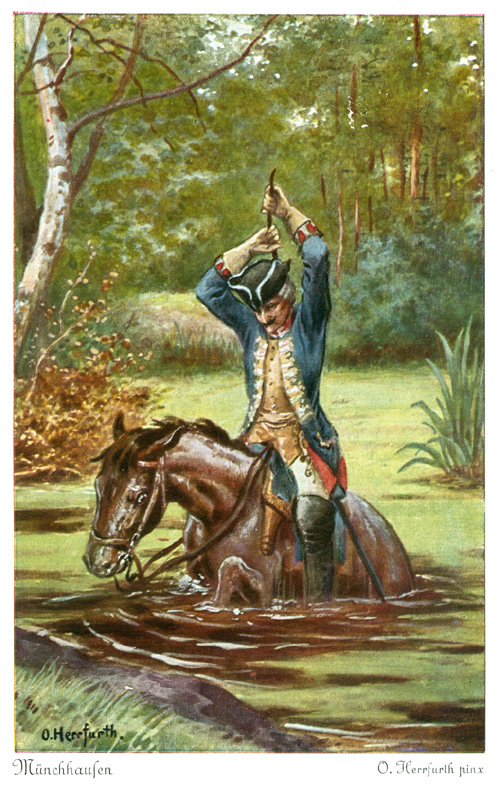
\includegraphics[width=3in]{munchausen.jpg}  \\
  \caption{The Great Baron Munchausen pulling himself up}
\end{figure}

\noindent
Here's a question you might ask: How many point of $S$ are left {\bf out} of each bootstrap sample, typically?
Answer: About a third.
\\~\\
{\bf Exercise.} 
Show that, for $m$ large, about $37\%$ of data points are left out of a
bootstrap sample created from $S$.






\section{Bagging}

The idea of Bootstrap samples can be used whenever we would like to create new
artificial samples from our only training sample $S$. It has many uses
throughout machine learning, statistics and data science. 
{\bf Bagging} is a nickname for a straightforward use of the Boostrap in machine learning, to
improve accuracy of an existing supervised machine learning algorithm.
\\~\\
 We start with a ``base''
learning algorithm $\Ac$ and a training sample $S$. We choose $T$ (later we'll
discuss how to choose it) and form
$T$ bootstrap training samples, $S^{*1},\ldots, S^{*T}$, each of size $m$. We
then train our learner {\bf separately} on each of the $T$ bootstrap training samples.
We form the committee $h_{S^{*1}},\ldots,h_{S^{*T}}$. We store all $T$ trained
models. When we need to classify a new test sample $x\in\X$,
we run $x$ through all the rules and classify using the 
majority vote of the committee,
\[
  h_{bag}(x) := sign\left( \sum_{t=1}^T h_{S^{*t}} (x)\right)
\]

For example, if we run Bagging on top of the Decision Tree classifier, we'll
obtain a committee of decision trees:
\begin{figure}[H]
  \centering
  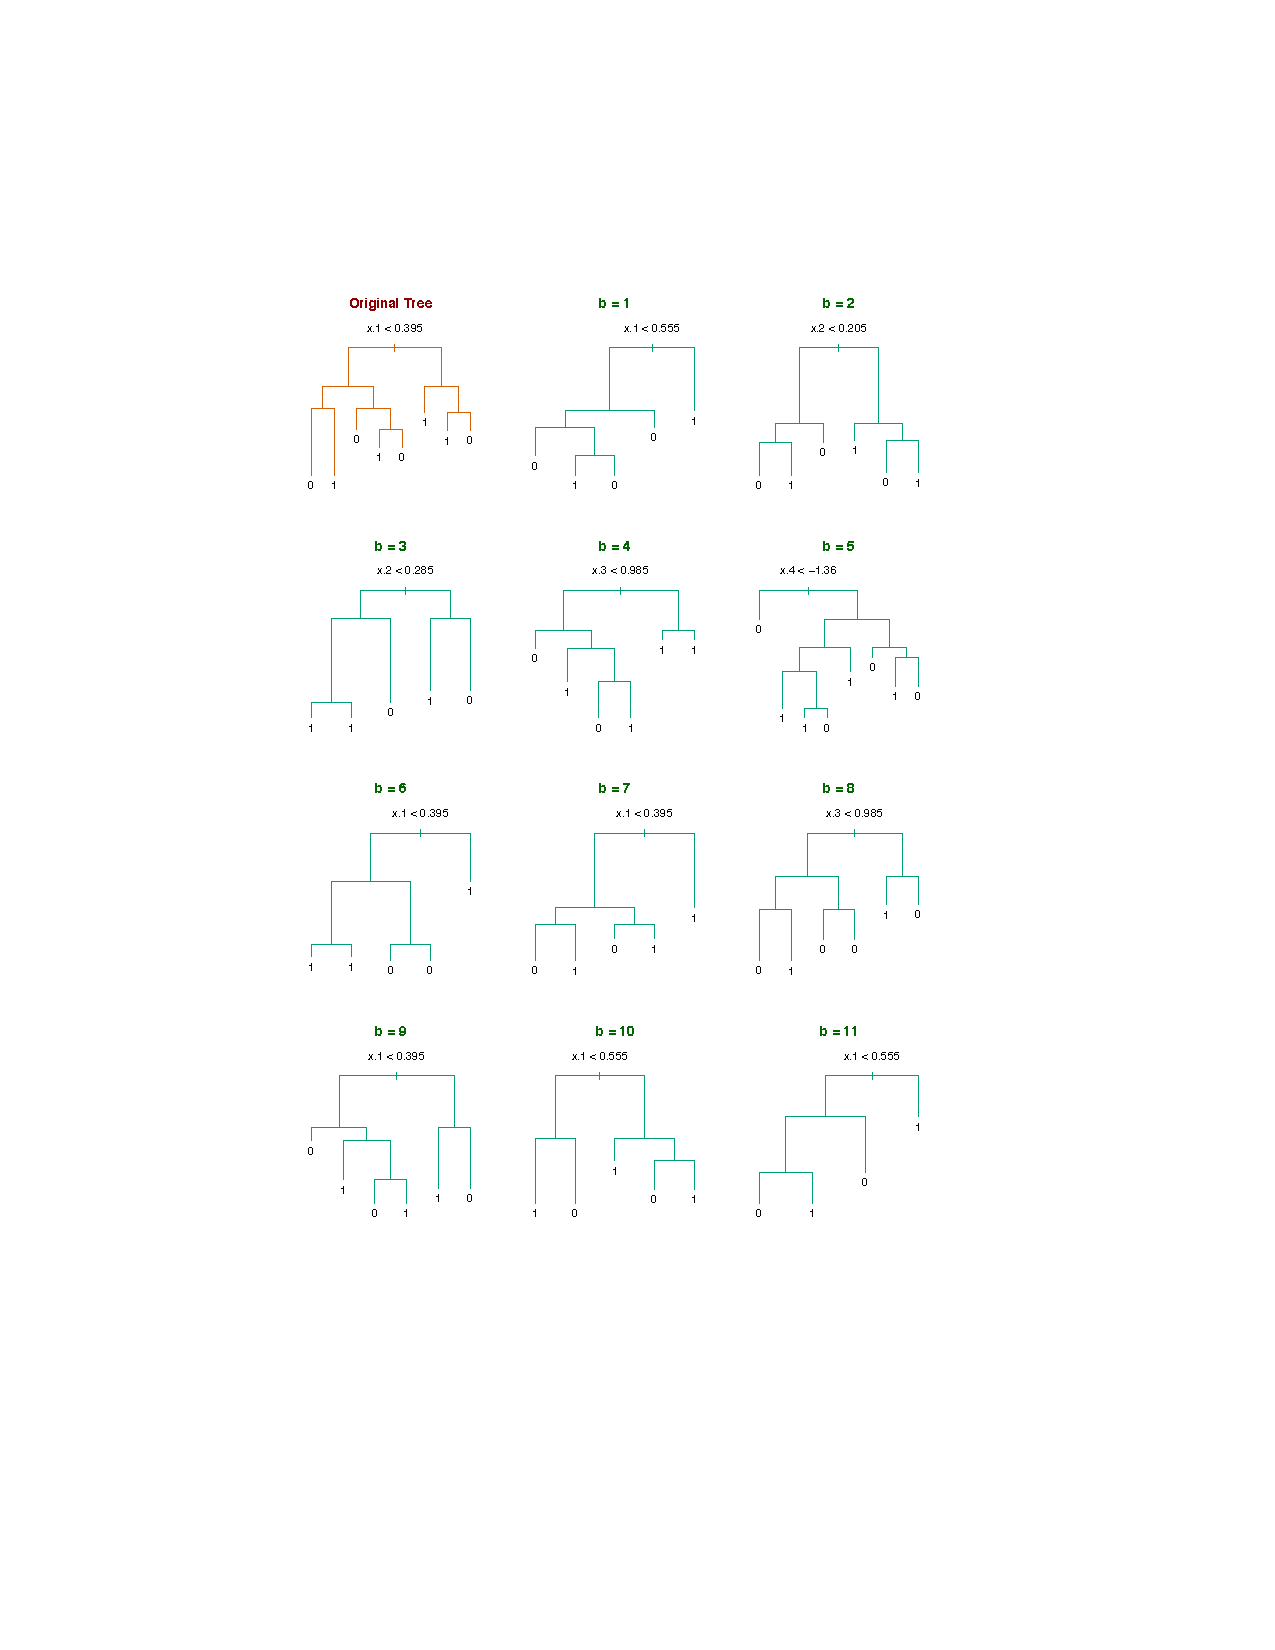
\includegraphics[width=3in]{many_trees.pdf}
  \caption{Collection of Bagged Decision Trees. (Source: ESL)}
\end{figure}





\paragraph{Handling repeated samples.} 
Note that our learner $\Ac$ must know how to handle repeated samples. We may have them
anyway in $S$, but running on a bootstrap sample we are sure to have them. Some
learning algorithms don't like repeated samples - as they cause numerical
problems (for example, linear and logistic regression.) Some really don't care
(for example, decision trees and $k$-NN).


\subsection{This is shockingly effective}

Does Bagging a learning algorithm reduce its generalization error? This is what
the original paper observed:
\begin{figure}[H]
  \centering
  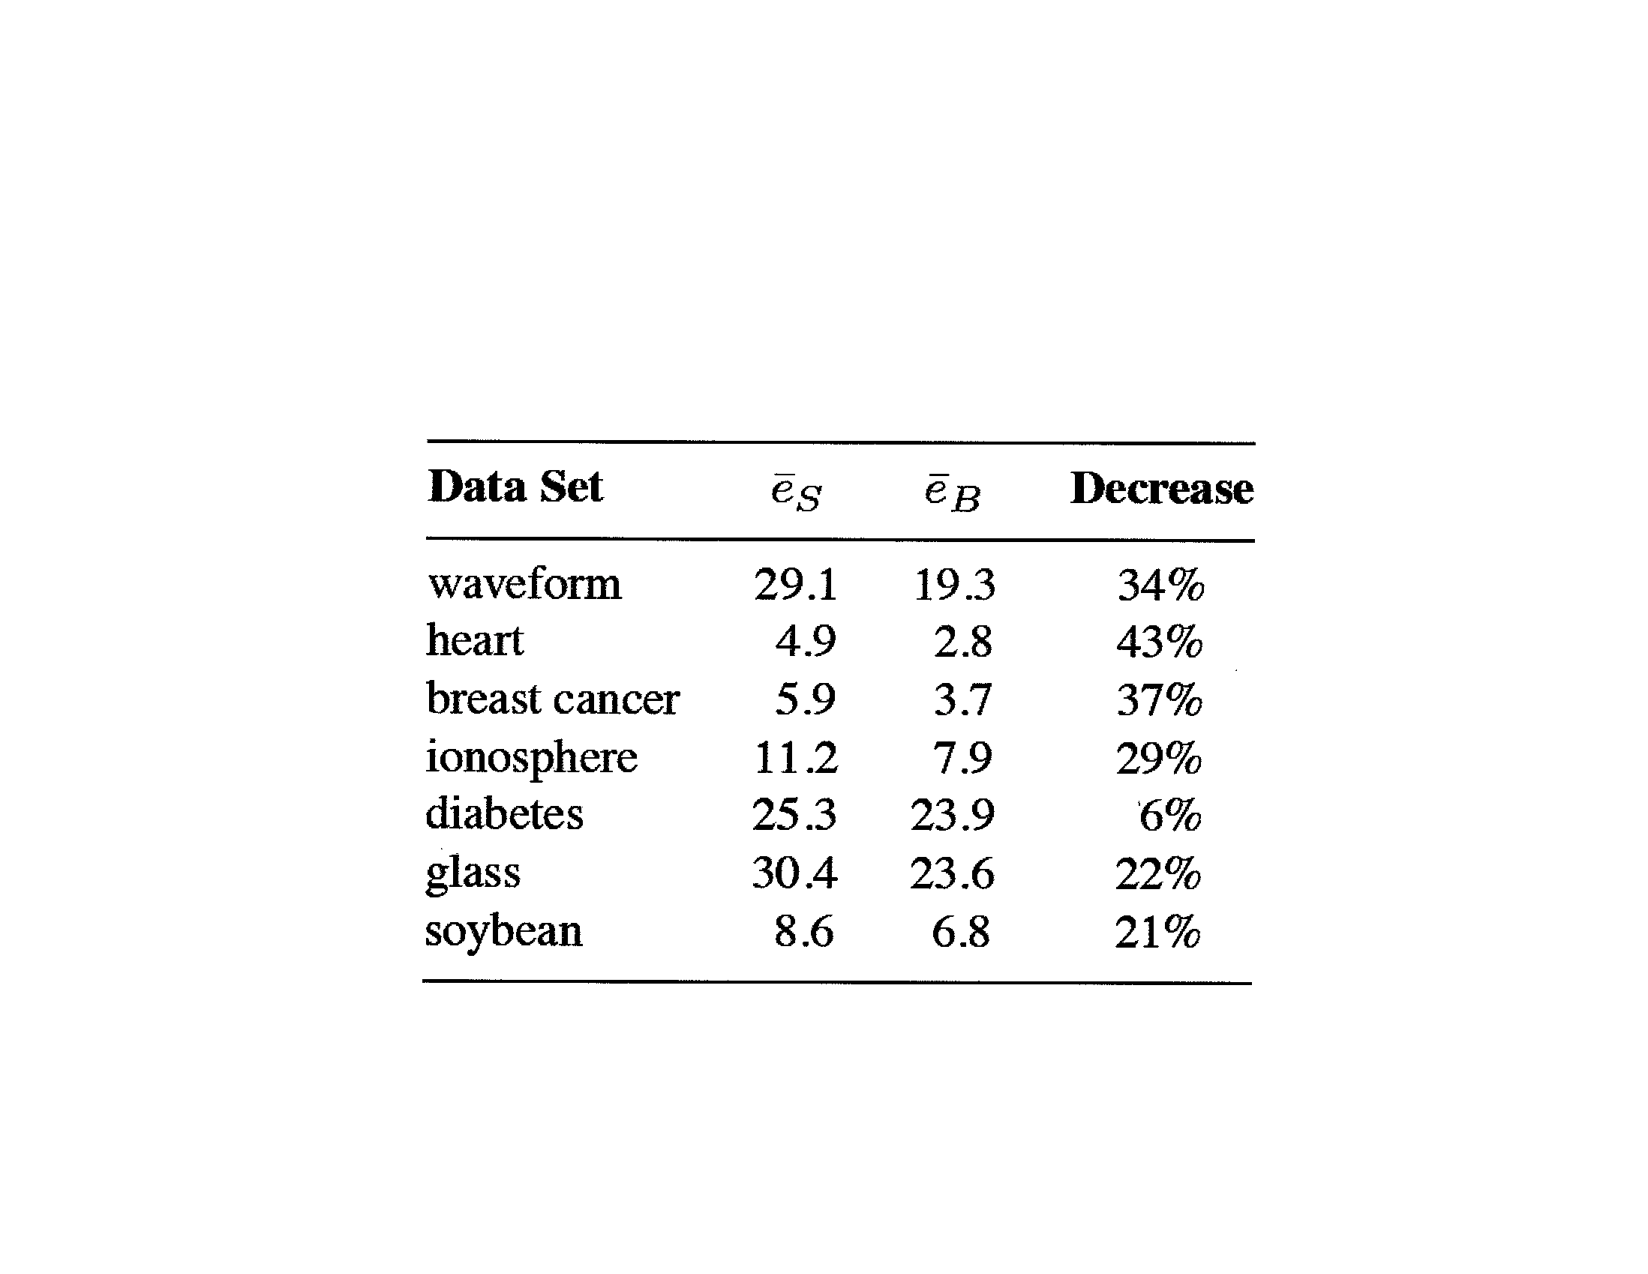
\includegraphics[width=3in]{breiman.pdf}
  \caption{Improvement of Bagging Decision Trees over a single tree. From the
    original paper \emph{
  Shang and Breiman,  Distribution Based Trees Are More Accurate}}
  \label{breiman}
\end{figure}

\noindent So a simple and straightforward trick can hugely reduce generalization risk.

\begin{figure}[H]
  \centering
  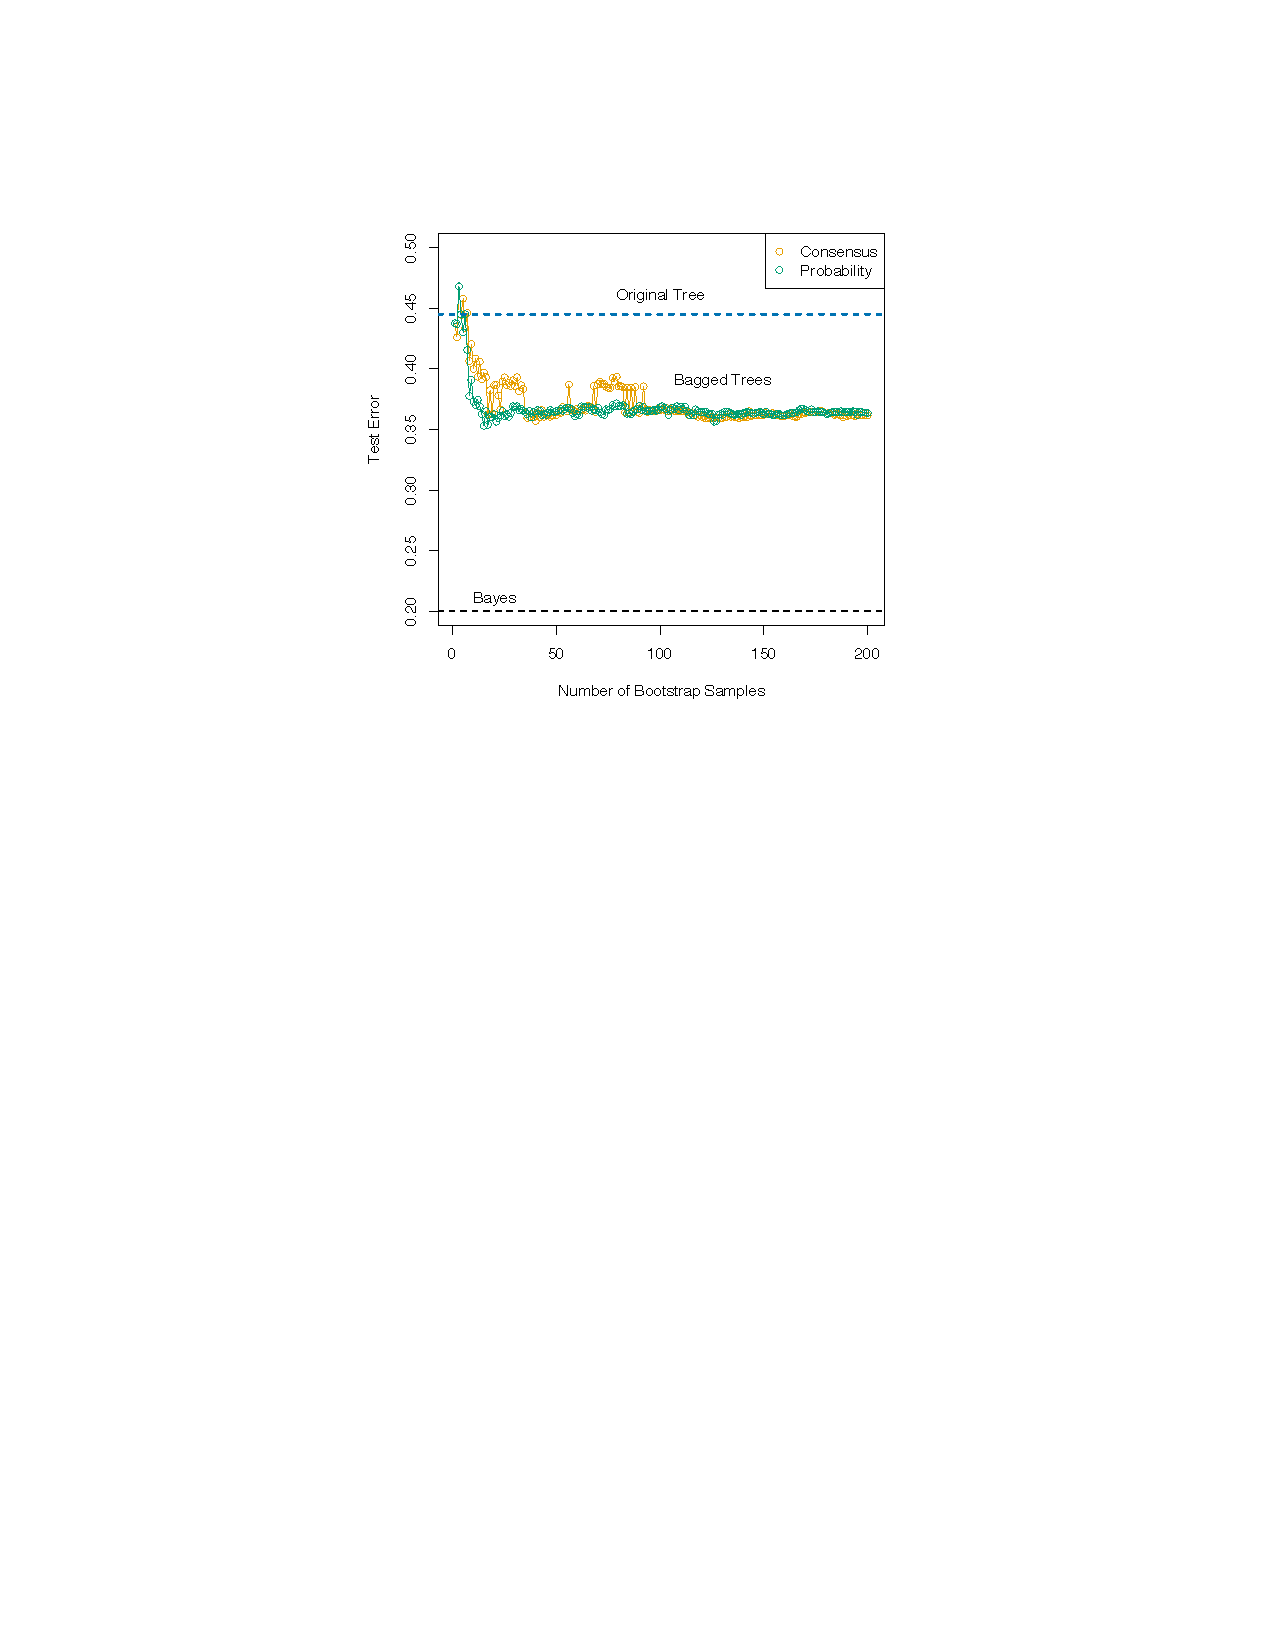
\includegraphics[width=4in]{bagging_trees.pdf}
  \caption{Test error of simple Bagging of decision trees, over $T$ the number
    of bagged trees (Source: ESL)}
\end{figure}


\subsection{Bagging reduces variance}

We saw that a committee majority vote reduces variance - but only to a certain
degree, which is determined by the correlation between committee members. So, we
can expect bagging to reduce variance as $T$ increases - and therefore to reduce
the generalization error - but only to a certain degree, determined by the
correlation between the bagged prediction rules. So, Bagging can be improved by
somehow de-correlating the bagged prediction rules.

\subsection{Decorrelation}

How do we de-correlate the committee
members - namely, cause their predictions somehow to be less correlated? One way to
do this is by handicapping (restricting) each learner a little, in a random way, and hope that
the performance gain (in bagging them) due to de-correlation is more than the
performance loss to each learner by handicapping. The most well know example of
this principle is {\bf Random Forests.}




\subsection{Random Forest: Bagging of Decision Trees + De-correlation}

Recall the Decision Tree classification algorithm over $\X=\R^d$. We have a
training sample $S$ with $m$ points. 
The Random Forest classifier is obtained by using Bagging on top of 
the Decision Tree algorithm, {\bf with an important
twist} for de-correlation: the algorithm has a tuning parameter $k\leq d$. When
growing each decision tree, in each split, we choose $k$ out of the $d$
coordinate uniformly at random, and only choose the split among these $k$
coordinates. Formally:

\begin{itemize}
  \item The tuning parameters are:
    
    \begin{itemize}
      \item $R\in \mathbb{N}$, the maximum depth of each
    tree
  \item  $m_{min}$, the minimal number of training samples in any leaf of any
    of the trees
  \item $T$, the number of Bagging samples (number of trees in the
    forest)
  \item $k$, the number of coordinates allows in choosing each split.
  \item  (There is an additional tuning parameter for {\bf pruning} a decision tree
    which we'll discuss in a future lecture.) 
    \end{itemize}
  \item For each $t=1\ldots T$:
    \begin{itemize}
      \item Draw a Bootstrap sample $S^{*t}$ from $S$
      \item Train a decision tree $h_{S^{*t}}$ on the sample  $S^{*t}$. While
        growing the tree, in each
        split do the following:
        \begin{itemize}
          \item Select $k$ coordinates from $\left\{ 1,\ldots d \right\}$
            uniformly at random
          \item Pick the best (coordinate,split-point) combination using only
            the $k$ coordinates chosen
          \item Split on the best combination 
        \end{itemize}
      \item Do not split a box if the maximal depth $R$ or the minimal number of
        training samples $m_{min}$ are reached.
    \end{itemize}
  \item Output the grown trees $h_{S^{*1}},\ldots ,h_{S^{*T}}$.
   \end{itemize}

\noindent
This de-correlation trick works: pretty much on every classification problem
you'll work on, you'll observe something like the next plot: Bagging trees is
much better than a single tree, and Random Forest (Bagging with the
de-correlation trick) is better than just Bagging trees. (And, sometimes,
Boosting trees is better than both - but we're coming up to that.)


\begin{figure}[H]
  \centering
  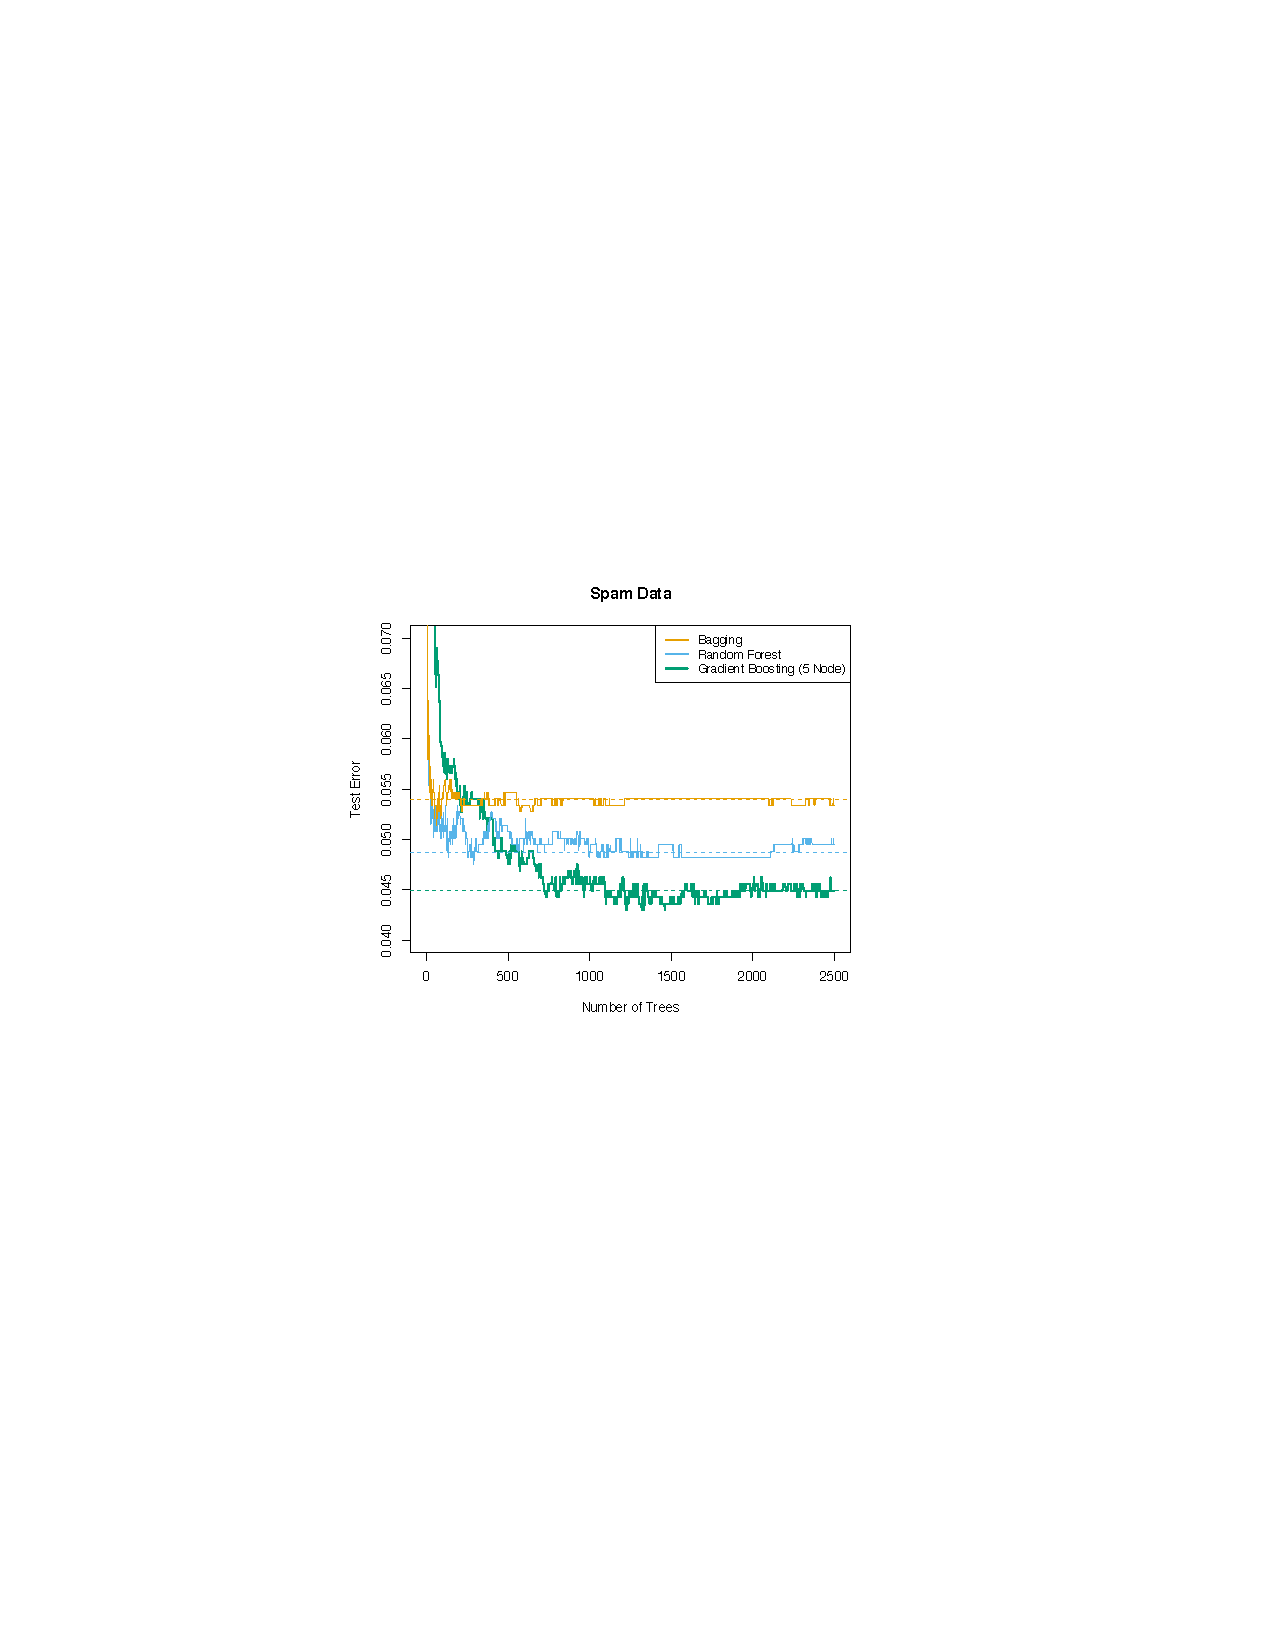
\includegraphics[width=4in]{bagging_vs_rf.pdf}
  \caption{Test error of simple Bagging of decision trees (no de-correlation),
  Random Forests, and Gradient Boosting of Trees. (Source: ESL)}
\end{figure}

\subsection{Some discussion points about Bagging}

\subsubsection*{Can Bagging hurt us?}

Always remember that a committee of fools (a committee where each member has
probability $p<0.5$ to make the right decision) makes worse decisions than a
single member. So, when our base learner is so poor that its generalization loss
is less
than $0.5$ we shouldn't use Bagging.

\subsubsection*{What are the disadvantages of Bagging?}

\begin{itemize}
  \item We need to train $T$ models, not just one
  \item For prediction on new samples, we need to store $T$ models, not just one
  \item Loss of interpretability: it's harder to understand why the committee
    made a decision - we need to understand the decision of each of the $T$
    members
\end{itemize}

\subsubsection*{Bagging and predicted class probabilities}

\noindent 
Question: Can we use the {\bf proportion} of the committee members who voted
$+1$ as a predicted class probability? 
\\~\\
Answer: It's not a good idea. Estimated class probabilities are estimates of 
$\prob\left\{ Y=+1,|\, X=x \right\}$. The proportion of  members who voted
$+1$ estimates $\prob\left\{ h_S(x)=+1 \right\}$, which is a different quantity.


\subsubsection*{Parallel implementation of Bagging and Random Forests}

From the computational perspective, it is important to note 
that Bagging in general (and Random Forests in particular) is {\bf embarrassingly
parallelizable}. When training a Bagging model with $T$ committee members, we
can use $T$ machines in parallel, each using its own random seed to select
Bootstrap samples (and random splits, in Random Forest). The machines do not
need to interact; when each machine is done, it returns the committee member
$h_t$ to the master node. 


\subsubsection*{Decision boundary in bagging}

\begin{figure}[H]
  \centering
  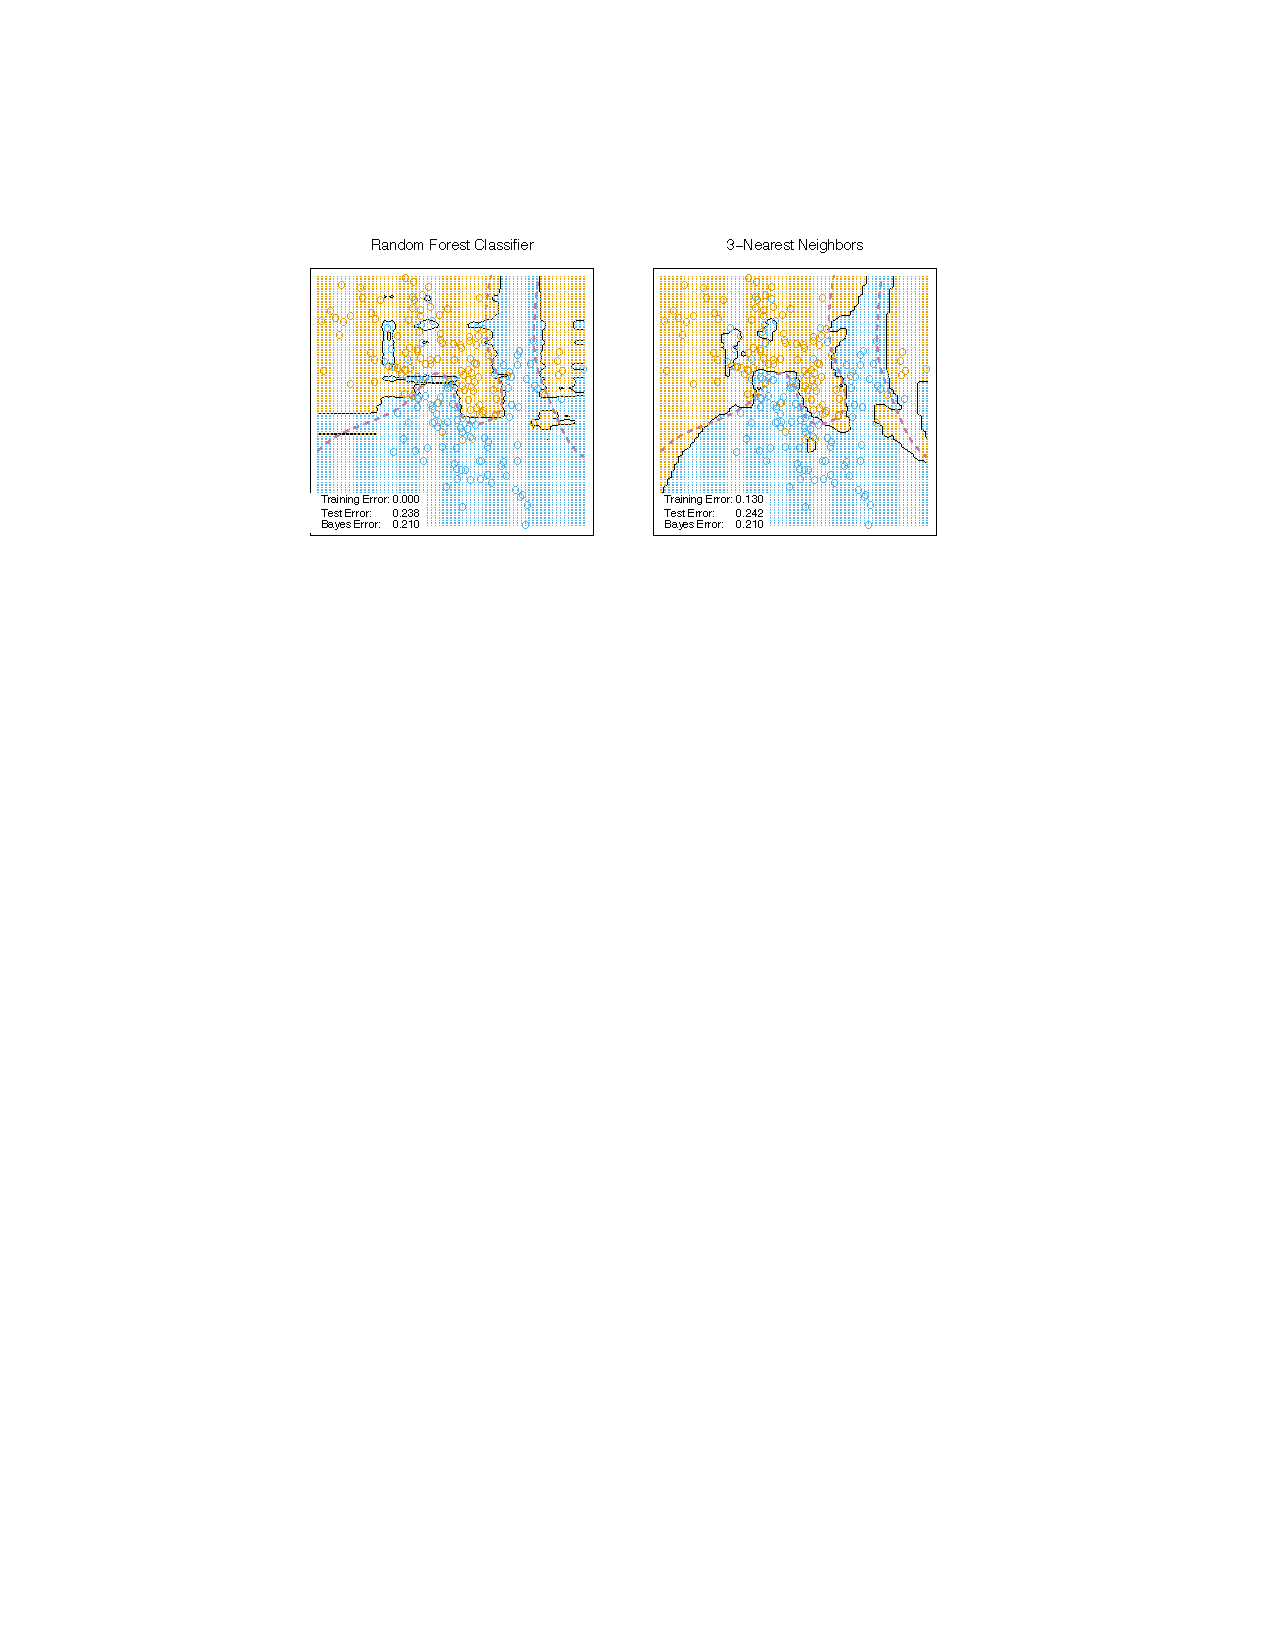
\includegraphics[width=5in]{rf_decision.pdf}
  \caption{Left: Decision boundary of a Random Forest classifier. Right:
  Decision boundary of a $3-NN$ classifier. Observe that the Random Forest tends
to have axis-parallel boundaries. (Source: ESL)}
\end{figure}

\subsection{Random Forest classifier summary}

Random Forest is a very popular classifier. As it doesn't overfit for $T$
(number of trees) too large, we just try to avoid making $T$ too large for
efficiency reasons. For choosing $k$ (the number of random coordinates allowed
for each split), the rule of thumb is $k:=\sqrt{d}$ where $d$ the ambient
  dimension, $\X=\R^d$. 
\\~\\
{\bf Exercise:} Complete the following summary of the Random Forest Classifier
(note that we still didn't learn how to {\bf prune} each decision tree in the forest.)

\begin{itemize}
  \item Hypothesis class 
       \item Learning principle for training model (choosing $f\in\Hc$):
	     \item Computational implementation of learning principle:
  \item How to make predictions on new samples:  
  \item Interpretable
    \item Estimates class probabilities 
    \item Family of models
       \item Time complexity for training, and for predicting on a new sample
  \item How to store trained model
\end{itemize}

\section{Boosting}

Bootstrap was magic of the following kind: we take a single
training sample $S$ and turn it into many training samples. Bagging uses this
magic by training a model over these ``new'' training samples, and averaging the
result to reduce the variance and hence the generalization error.
\\~\\
Boosting is magic of a different kind. In Boosting we take a ``weak'' learning
algorithm - an algorithm with better-than-random but possibly not so good accuracy (accuracy = generalization error) and {\bf
boost} it - using a clever committee method - to obtain a learning algorithm
with good accuracy. 
\\~\\
The core magical idea of Boosting is a completely different idea for creating a committee of prediction
rule from a base learning algorithm
$\Ac$ and a single training sample $S$. 
In Bagging, we ``pretended'' to have fresh training samples $S_1,\ldots,
S_T$, and each committee member trained on a different sample. In Boosting, we go
even further and ``pretend'' to have {\bf different underlying distributions $\D$
from which the training sample is drawn}.
\\~\\
More specifically, in Boosting each committee member $h_t$ is the result of
running $\Ac$ against a training sample $S_t$ that mimics an i.i.d sample of
size $m$ 
from a {\bf different distribution} $D^t$. Whereas in Bagging each committee
member is trained independently of all other members, in Boosting the committee
members are trained sequentially - one after the other - and each is an
improvement, in some sense, on the previous one. 
\\~\\
The clever idea behind Boosting is that after we finish training $h_t$, based on
the distribution $D^t$, 
we
update the distribution in a way that {\bf increases the distribution at training
samples where $h_t$ was wrong}. This way, $h_{t+1}$ will try very hard not to be
wrong on those particular samples, and so on. 
\\~\\
Here is a cartoon of how Boosting iterations progress:
\begin{figure}[H]
  \centering
  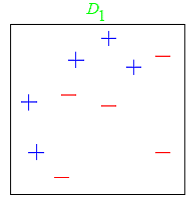
\includegraphics[width=2in]{boosting_toy0.png}
  \caption{Original problem. Uniform distribution $D^1$.}
\end{figure}
\begin{figure}[H]
  \centering
  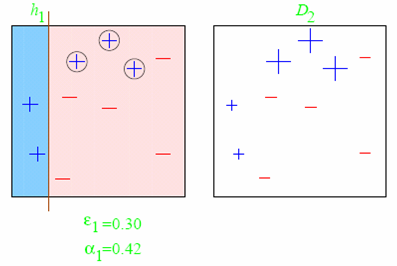
\includegraphics[width=2.5in]{boosting_toy1.png}
  \caption{Iteration $1$. Left: $h_1$ with $D^1$. Right: $D^2$ }

\end{figure}
\begin{figure}[H]
  \centering
  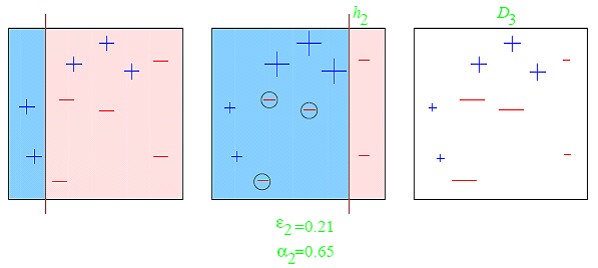
\includegraphics[width=4in]{boosting_toy2.png}
  \caption{Iteration $2$.  Left: $h_1$ with $D^1$. Center:
  $h_2$ with $D^2$. Right: $D^3$}
\end{figure}
\begin{figure}[H]
  \centering
  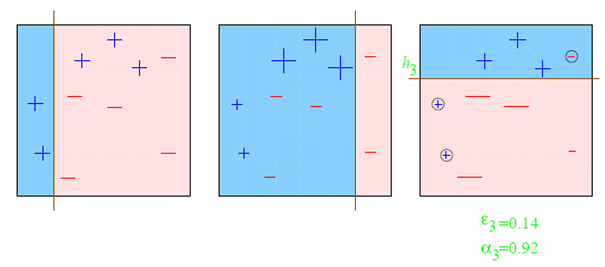
\includegraphics[width=4in]{boosting_toy3.png}
  \caption{Iterations $3$. Left: $h_1$ with $D^1$. 
  Center: $h_2$ with $D^2$. Right: $h^3$ with $D^3$}
\end{figure}
\begin{figure}[H]
  \centering
  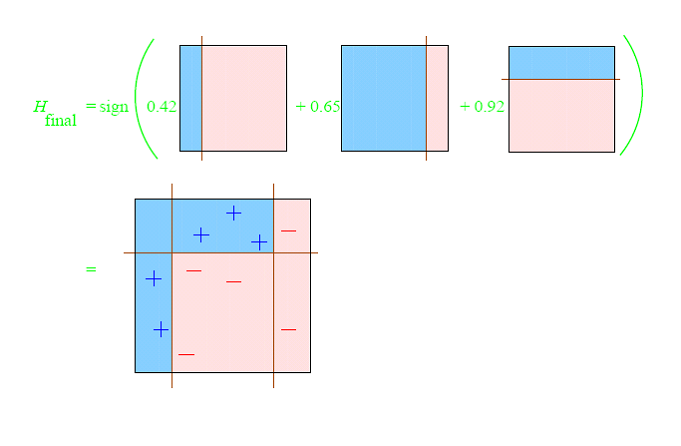
\includegraphics[width=5in]{boosting_final.png}
  \caption{The Boosting committee}
\end{figure}



\subsection{Classification problem with a weighted sample}

But first, we have to understand  what is meant, exactly,  by ``running $\Ac$
against the training sample $S$ with distribution $D^t$''.  
\\~\\
One way to interpret this is to take a {\bf weighted Bootstrap} sample from $S$,
where the probability of selecting $(x,y)\in S$ is proportional to $D^t(x,y)$. 
\\~\\
A simpler way to interpret this is as follows. If $\Ac$ uses the ERM principle,
say for standard misclassification ($0-1$ loss),
namely, looking to minimize the empirical risk,
\[
  L_S(h) = \sum_{i=1}^m \mathbf{1}_{[y_i \neq h(x_i)]} 
\]
then we can use $S$ itself (not
any bootstrap sample) and have the base learner 
minimize the {\bf weighted} empirical risk
\[
  L_{S,D^t}(h) = \sum_{i=1}^m D^t_i\mathbf{1}_{[y_i \neq h(x_i)]} 
\]
where for each $(x_i,y_i)\in S$ we write $D^t_i := D^t(x_i,y_i)$, so that  
$\sum_{i=1}^m D^t_i =1$.
\\~\\
Observe that these two interpretations are equivalent in expectation. Indeed,
the expected number of times for a sample $(x_i,y_i)$ to appear in the weighted
Bootstrap sample is $D^t_i$, and so it would (in expectation) appear $D^t_i)$
times in the empirical risk sum. 
\\~\\
Note that we usually prefer second option (using weighted empirical risk) to the
first option (using weighted bootstrap). 
It's more computationally efficient, and does not require worrying about
repeated samples.
However, the first option (using weighted bootstrap) is always available. The
second option (using weighted empirical risk) is not always possible, and is
implemented ad-hoc for the particular base learner we are boosting.
\\~\\
{\bf Exercise:}
To help you understand this point, describe how you would implement a Decision
Tree with each of the two methods:
\begin{itemize}
  \item Using weighted empirical risk: How would you change the Decision Tree
    algorithm we've seen (CART) to work with a given weight vector $D^t$ over
    the training sample $S$? (Hint: what is the best splitting now that we have
    weights?)
  \item Using weighted Bootstrap: How would you How would you change the Decision Tree
    algorithm we've seen (CART)  to work with a given weight vector without
    changing the splitting algorithm, namely, by giving the algorithm a
    different training sample selected by weighted Bootstrap? Will the algorithm
    work with repeated samples?
\end{itemize}
~\\
It is much less trivial to adapt learning algorithms that do not use the ERM
principle. For example, Soft SVM can be adapted to work with weights, 
by penalizing the slack
variables - but this is not trivial\footnote{Look for ``boosting support vector
machines.''}.



\subsection{Adaboost}

There are many Boosting meta-algorithms. The one we will learn here was the
original one, known as {\bf Adaboost} (for ``{\bf Ada}ptive {\bf Boost}ing'')
\\~\\
Adaboost, as a form of boosting, is characterized as by the following statements:
\begin{itemize}
  \item Set the initial distribution to be uniform, $D^1_i=1/m$, $i=1,\ldots,m$
  \item Use exponential updates for the distribution
    \[
      D^{t+1}_i \leftarrow \frac{D^t_i \cdot e^{-w_t y_i h_t(x_i)} }
      {\sum_{j=1}^m  D^t_j \cdot e^{-w_t y_j h_t(x_j)} }
    \]
    for some {\bf exponent} $w_t>0$. (Notice how if point  $i$ is classified
      correctly then $ y_i h_t(x_i)=1$,  so its weight goes down in the next
      iteration. Conversely, if point  $i$ is classified
    incorrectly then $ y_i h_t(x_i)=-1$,  so its weight goes up.)
  \item Choose the exponent $w_t$ exactly such that
    \[
      \sum_{i=1}^m D^{t+1}_i\mathbf{1}_{[y_i \neq h_t(x_i)]} = \frac{1}{2}\,.
    \]
    (We'll soon discuss why.)
  \item Each committee member $h_t$ votes with weight $w_t$, so that the
    label predicted by the committee is
    \[
      h_{boost}(x) := sign\left( \sum_{t=1}^T w_t h_t(x) \right)
    \]
\end{itemize}
~\\
The idea is simple: from iteration $t$ to iteration $t+1$, we want to {\bf
increase}
the weights of samples misclassified  by $h_t$ (where $y_i h_t(x_i)=-1$) and {\bf decrease}
the weights of samples correctly classified by $h_t$. We want to make the
classification problem ``maximally hard'' in the sense that weighted empirical
risk of $h_t$, with respect to the updated weights $D^{t+1}$, is the worse
possible, namely $1/2$.
Finally, the prediction rules vote in the committee with weights $w_t$.
\\~\\
\noindent{\bf Claim:}
The exponent we are looking for is
\[
  w_t := \frac{1}{2}\log\left( \frac{1}{\epsilon_t} -1 \right)
\]
where $ \epsilon_t = \sum_{i=1}^m D^t_i\mathbf{1}_{[y_i \neq h(x_i)]} $ is the
weighted empirical risk of $h_t$.
\\~\\
{\bf Proof:} \begin{align*}
  &\sum_{i=1}^m D^{t+1}_i \, \mathbf{1}_{[y_i \neq h_t(\x_i)]}  =  \frac{ \sum_{i=1}^m
	D^t_i \, e^{-\w_ty_ih_t(\x_i)}
      \mathbf{1}_{[y_i \neq h_t(\x_i)]} }{\sum_{j=1}^{m}D^t_j e^{-\w_t
    y_jh_t(\x_j)} }\\
&\\ 
&=  \frac{ e^{\w_t} \epsilon_t }{e^{\w_t} \epsilon_t  + e^{-\w_t}
  (1-\epsilon_t ) } =  \frac{  \epsilon_t }{ \epsilon_t + e^{-2\w_t}
  (1-\epsilon_t) }
&\\ 
&=  \frac{  \epsilon_t }{ \epsilon_t +
  \frac{\epsilon_t}{1-\epsilon_t} (1-\epsilon_t) } ~=~ \frac{1}{2}~. 
\end{align*}
~\\
You may be wondering why the right weights for the committee votes are given by
the same exponents $w_t$ we used to update the distribution. This will become
clear next.
%question: given number of iterations $b$ and running time of weak learner, 
%what's the running time of Adaboost?
\\
~\\
To recap, here is the Adaboost meta-algorithm:
\begin{itemize}
\item \textbf{input:} training set $S=(\x_1,y_1),\ldots,(\x_m,y_m)$;
  base (``weak'') learner $\Ac$ that takes both a training sample of size $m$ and a
  distribution on $m$ points; number of rounds $T$.
\item \textbf{initialize} $D^1= (\frac{1}{m},\ldots,\frac{1}{m})$
\item \textbf{for} $t=1,\ldots,T$
\begin{itemize}
\item   invoke base learner $h_t = \Ac(D^t,S)$
\item compute $\epsilon_t = \sum_{i=1}^m D^t_i
  \, \mathbf{1}_{[y_i \neq h_t(\x_i)]} $ 
\item let $w_t:=\frac{1}{2}\log\left(\frac{1}{\epsilon_t}-1\right)$
\item update $D^{t+1}_i = \frac{D^t_i
    \exp(-w_ty_ih_t(\x_i))}{\sum_{j=1}^{m}D^t_j\exp(-w_t
    y_jh_t(\x_j))}$
  for all $i=1,\ldots,m$ 
\end{itemize}
\item \textbf{output} the hypothesis $h_{boost}(\x)=sign\left(\sum_{t=1}^{T} w_t
    h_t(\x)\right)$.
\end{itemize}


\subsection{PAC view of boosting}


Historically, Boosting appeared as an answer to a fascinating question. Let us
formulate this question in PAC framework.

\begin{definition}[$\gamma$-weak-learner]  ~
A learning algorithm $\Ac$ is
a $\gamma$-weak-learner for an hypothesis class $\Hc$ 
if there exists a function $m_\Hc:(0,1)\to\mathbb{N}$ such that for every
$0<\delta<1$, for every distribution $\D$ over the sample space $\X$, and for
every labeling function $f:\X\to\left\{ \pm \right\}$, if the realizabiity
assumption holds with respect to $\Hc,\D,f$, then when running $\Ac$ on a
training sample of $m\geq m_\Hc(0,1)$ i.i.d samples drawn according to $\D$ and
labeled by $f$, the algorithm returns an hypothesis $h_S=\Ac(S)$ such that wwith
probability at least $1-\delta$ (with respect to choice of the training sample
$S$), we have $L_{\D,f} (h_S) \leq 1/2-\gamma$. 
\\~\\
An hypothesis class $\Hc$ is $\gamma$-weak-learnable if there exists a
$\gamma$-weak-learner for $\Hc$. 
\end{definition}
~\\
How is this different than PAC-learnability? If an hypothesis class $\Hc$ 
is PAC-learnable, then for {\bf every} $(\epsilon,\delta)$ there exists a
learner $\Ac$. This means that we can learn and generalize a labeling function
from $\Hc$ to any accuracy $\epsilon$ we want. But if $\Hc$ is
$\gamma$-weak-learnable, for any $\delta$ {\bf and just for
$\epsilon=1/2-\gamma$}
there is a learner $\Ac$.
We may not be able to find a learner that has better
accuracy (lower
$\epsilon$). 
\\~\\
The question that motivated Boosting was the following: 
\begin{itemize}
  \item Suppose that $\Hc$ is PAC-learnable. Then we know that the rule
    $ERM_{\Hc}$ will learn (namely, will be probably approximately correct etc)
    with a near-minimal number of samples.
  \item But what if $ERM_\Hc$ is computationally hard? (we've seen examples)
  \item Assume we can find a {\bf simple} hypothesis class (a ``base hypothesis class'')
    $\Hc_{base}$, such that $ERM_{\Hc_{base}}$ 
    (choosing the hypothesis in $\Hc_{base}$ with lowest empirical risk) is
    computationally efficient, and is
    $\gamma$-weak-learner for $\Hc$ for some $\gamma$.
  \item This means that we have a computationally efficient way to learn with
    accuracy $1/2-\gamma$, for some $\gamma$. Maybe we can't 
    find an efficient learner with better $\gamma$.
  \item Is there a way to {\bf boost} $ERM_{\Hc_{base}}$ in a computationally
    efficient way, 
  and create a computationally efficient learner $\Ac$ 
  which is close to minimizing $ERM$ over $\Hc$?
\end{itemize}
~\\
For example, think about Decision trees. We saw that the ERM learner is not
computationally feasible on this hypothesis class. But a small tree may be able
to achieve accuracy (over a sample labeled by a larger tree)
which is not great, but better than random.
\\~\\
Well, as the following theorem shows, Adaboost does just that. (We won't prove
this theorem - you can see the proof in UML 10.2).
\\~\\
{\bf Theorem.} Let $S$ be a training set. 
Assume that at each iteration of
Adaboost, the base learner returns a prediction rule (hypothesis $h_t$) for which the
weighted empirical risk satisfies
\[
  \sum_{i=1}^m D^{t}_i\mathbf{1}_{[y_i \neq h(x_i)]} \leq \frac{1}{2}-\gamma\,.
\]
Then the (standard, non-weighted) 
empirical risk of the output prediction rule of Adaboost,
$h_{boost}$, (the weighted committee
vote) satisfies
\[
  L_S(h_{boost}) \equiv \frac{1}{m}\sum_{i=1}^m \mathbf{1}_{[y_i 
  \neq h_{boost}(x_i)]} \leq e^{-2\gamma^2 T }\,.
\]

%But how do we deduce that low training error implies low generalization loss?
%Recall from the proof of part 1 of the fundamental theorem that if $VCdim(\Hc)$
%is finite, then for every $\delta$ we can find large enough $m$ such that 
%\[
%  \Pr\left\{ S\in(\X\times\Y)^m \,\big|\, 
%  sup_{h\in\Hc} \big| L_\D(h) - L_S(h) \big| > \epsilon \right\} <\delta\,.
%\]
%(We even had a bound that used Markov's inequality and the growth function
%$\tau_\Hc$).
%
%So, the question is whether the VC-dimension of the hypothesis class of the
%weighted committee is not too large. 
%
%{\bf Theorem: The VC dimension of the committee is \dots}


%So, without stating this formally as a theorem, we see (informally, but with
%most of the details) that Adaboost allows us to take a weak learner - a learner
%$\Ac$ that can be probably correct to any specified confidence $\delta$ but only
%approximately correct to (potentially poor) accuracy $1/2-\gamma$, and  {\bf
%boost} its accuracy to create a strong learner, namely a learner that can be
%probably approximately correct to any specified confidence $\delta$ and accuracy
%$\epsilon$.
%
\subsection{Bias and variance in boosting}

The hope is, of course, that we're not overfitting, so that low empirical risk
will imply low generalization loss. 
\\~\\
Suppose we run $T$ iterations of Adaboost 
over a learner $\Ac_{base}$ that returns hypothesis from $\Hc_{base}$. 
What is the effective hypothesis class we have now, and how large is it?
\\~\\
Well, Adaboost with $T$ iterations will return a function from the hypothesis class  
\[
  \Hc_T = \left\{ x\mapsto \sum_{t=1}^Tw_t h_t(x) \,
  \Bigg| \,
w_1\ldots w_T\in[0,\infty),\,\, \sum_t w_t=1,\,\,
h_1\ldots,h_T\in\Hc_{base}\right\}
\]
namely convex combinations of hypotheses from $\Hc_{base}$.
So $\Hc_t$ becomes larger (contains more functions) as $T$ grows. But it 
doesn't grow too fast with $T$. 
\\~\\
For example, we have a canonical way to measure the ``size'' of $\Hc_T$.
While we won't go into the details, under certain conditions,
$VCdim(\Hc_T)$ is roughly $T\cdot VCdim(\Hc_{base})$. 
So we can expect Boosting to increase the variance (compared with the base
learner) as $T$ increases, but ``not too fast''. 
\\~\\
On the other hand, it's clear that Boosting decreases bias - that is obvious
from the fact that the empirical risk decreases as $T$ grows - indeed 
$\Hc_T$ is able to come closer and closer to the labeling function on the
training set. And the fact that empirical risk decreases {\bf exponentially} with 
$T$ tells us that bias decreases quite quickly.
\\~\\
Overall, Boosting typically decreases bias much faster than it increases
variance, which is why it typically improves generalization loss quite
dramatically.
\\~\\
Question for you: If we use $T$ too large, will boosting overfit? 


\subsection{It's often better to Boost very simple learners}
Very often we see that boosting ERM over 
a very simple base hypothesis class is better than boosting ERM over a
more complicated class. 
For example, here is the test error (number of misclassification errors on a test set
the algorithm has never seen) of boosting {\bf
Decision stumps} - Decision trees with a single split - over number of
iterations $T$, compared with the test error of a single stump, and with a
single large Decision tree:


\begin{figure}[H]
  \centering
  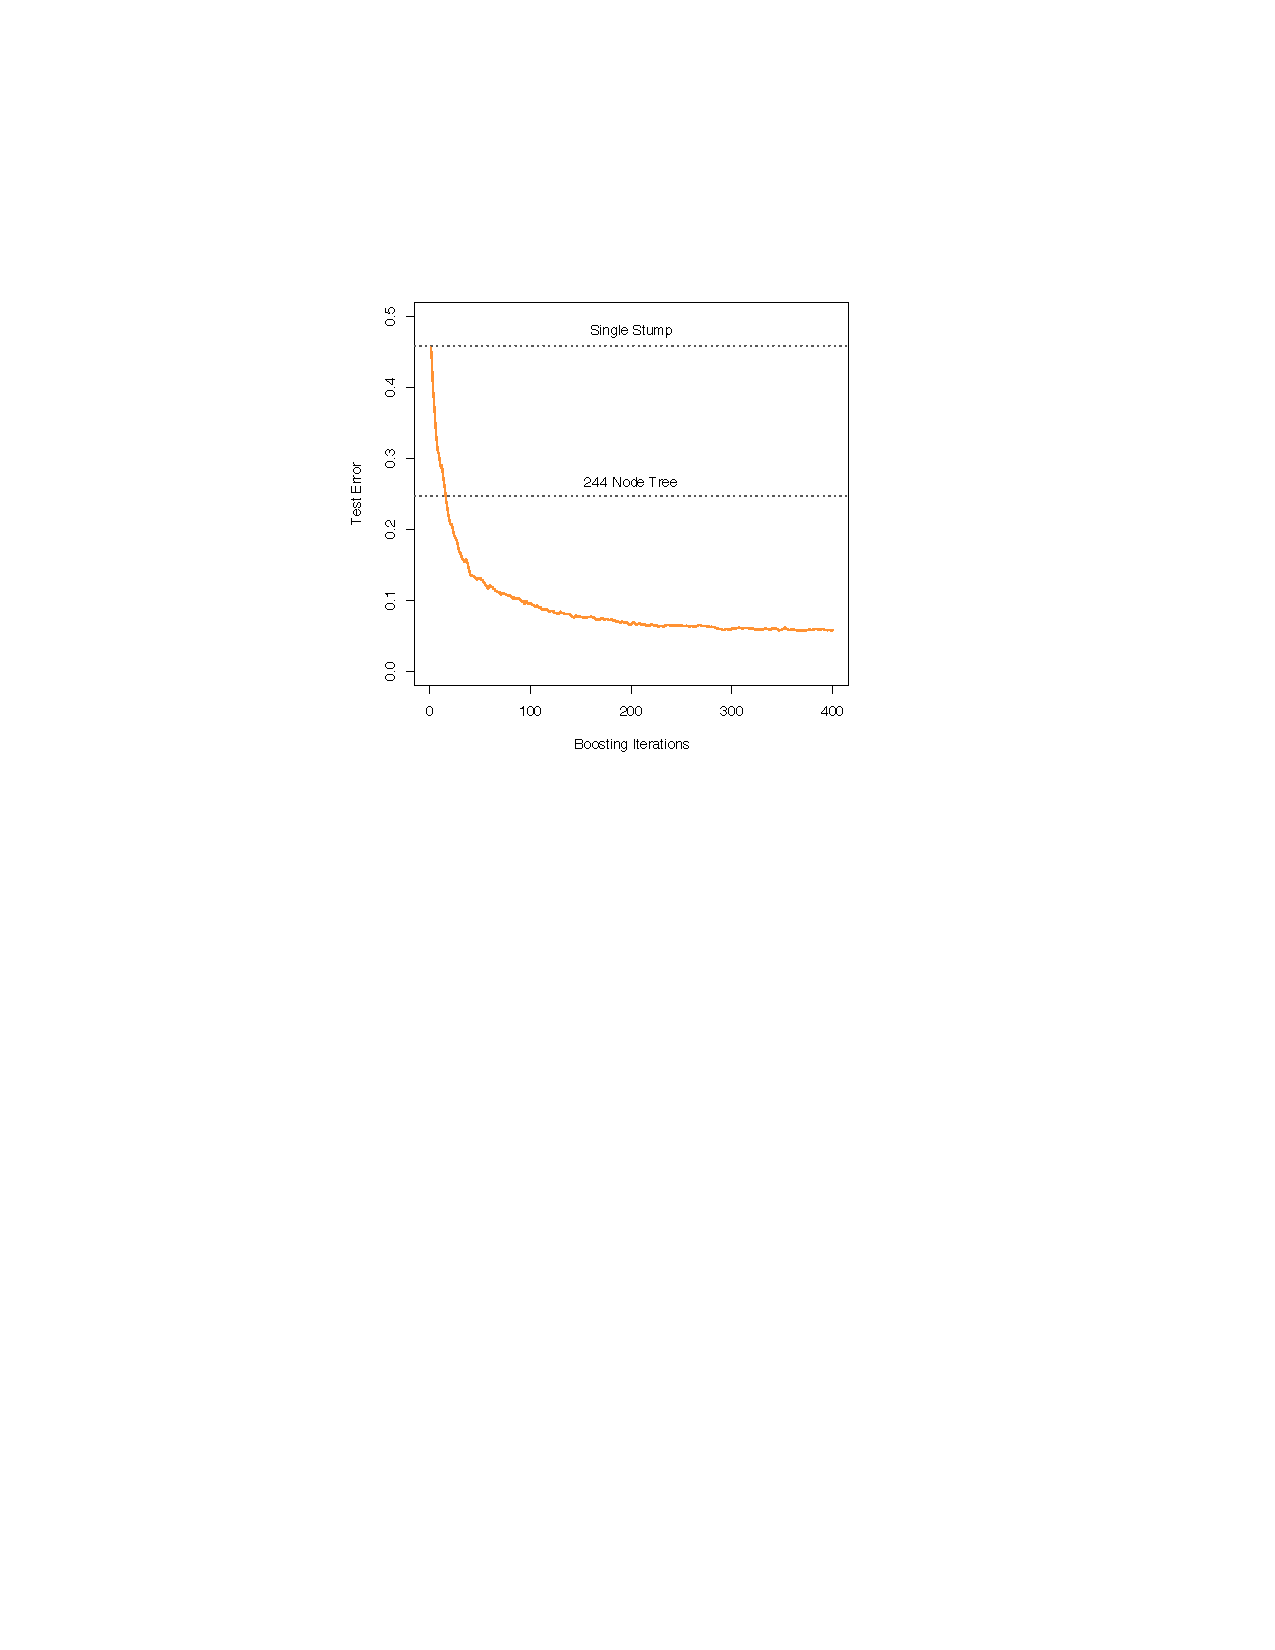
\includegraphics[width=4in]{adaboost_stumps.pdf}
  \caption{Test error of boosting decision stumps (single level decision
  trees), with Adaboost over the number of boosting iterations $T$.}
\end{figure}


%\subsection{Variable importance in Random Forests and Boosted Trees}\

%ryan boosting slide 18)
%\section{Statistical learning view of boosting}
%
%Boosting as additive logistic regression model.
%That is fitted with stagewise fitting (see Hastie slides and ESL p.305)
%
%Why exponential loss? smooth upper bound
%
%\subsection{Optimization view of boosting}
%
%Adaboost as coordinate descent of exponential loss function. Can replace with
%other losses as well.
%
%\subsection{Gradient boosting}
%
%\subsection{Boosting half-spaces VS SVM}
%
%
%\subsection{Boosting and interpretability}
%
%variable importance



\section{Bagging vs Boosting - Comparison}

Bagging and Boosting are both committee methods, but they are very different.
Let's compare them:

\begin{table}[H]
  \centering
  \begin{tabular}{|p{4.5cm}|p{5cm}|p{6.5cm}|}
    \hline
    & {\bf Bagging} & {\bf Boosting} \\
     \hline
      Learns committee members: & in parallel & sequentially \\
      \hline
      Dataset for each committee member: & bootstrap training samples
      & weighted bootstrap  {\bf or} original $S$ with weighted ERM\\
      \hline
      De-correlation: & recommended & not necessary \\
      \hline
      When $T$ is too large & Does not overfit & may overfit \\
      \hline
      Cause of improvement in generalization error: &
      reduces variance & reduces bias\\
      \hline
      With decision trees, use: & deep trees & shallow trees \\
      \hline
      Parallel compute implementation: & yes - easy & no \\
       \hline
      Committee vote: & unweighted & weighted \\
    \hline
  \end{tabular}
  \caption{Comparison of Bagging and Boosting}
\end{table}




\section{Summary}
We saw that a committee of learners using majority vote 
will have better accuracy than a single
member if each member is better than a random guess; the improvement in accuracy
due to the majority vote improves as the size of the committee grows, but is
bounded from below by the correlation between the members.
\\~\\
We saw three general methods:
\begin{itemize}
  \item {\bf Bootstrap} is a method for generating ``new'' training sample from
    the one training sample we have.
  \item {\bf Bagging} is a committee method where we run the learner against
    bootstrap samples. Learners are unrelated to each other. All have the same
    voting weight.
  \item {\bf Boosting} is a committee method where we run the learner
    sequentially on weighted bootstrap samples. The weights are larger for
    samples where we made a mistake in the last iteration. Learners vote with
    weights related to their empirical loss.
\end{itemize}
~\\
These methods implement three general principles: 
\begin{itemize}
  \item We can create ``artificial'' training sets from our one training set
    $S$ by sampling from $S$ with replacements. This method is known as {\bf The
    Bootstrap.} In a typical Bootstrap sample, about a third of the points a
    left out and others appear more than once. 
  \item We can create a learner with {\bf improved accuracy} and {\bf reduced
    variance} by averaging base
    learners. The base learners {\bf must} be better than a random guess. 
  When each base learner gets a Bootstrap training sample, this is called {\bf
  Bagging.} Bagging can be done in parallel as each prediction rule is created
  independently of the others. The prediction accuracy of the Bagging learner improves if the
    different prediction rules used are as de-correlated as possible.
    (Example: Random
    Forest is a classifier than achieves de-correlation by restricting each
  split in each tree to a random subset of coordinates.)
\item We can create a learner with with improved accuracy by {\bf boosting} a base
  learner. The key idea behind Boosting is working with a probability
  distribution over $S$. Boosting means creating a {\bf weighted} committee of prediction
  rules. Rules are created sequentially (not in parallel). Each rule is created the previous rule 
  by modifying the distribution in such a way that misclassified training
  samples get an increased weight. (Example: Adaboost is a Boosting method that
    uses exponential updates to the probability distribution on $S$, such that
    the weighted empirical risk of the previous rule according to the updated
  distribution is exactly $1/2$ - the worse it can be.)
\end{itemize}




